\documentclass[11pt, a4paper]{article}

\usepackage{geometry}
\geometry{left=2.54cm, right=2.54cm, top=2.20cm, bottom=2.20cm}

\usepackage[colorlinks=true, linkcolor=blue, urlcolor=blue, citecolor=blue]{hyperref}

\usepackage{fontspec}
\setmainfont{Times New Roman}

\usepackage{amsmath}
\usepackage{graphicx}
\usepackage{float}
\usepackage{caption}
\captionsetup{font=small, skip=3pt, belowskip=0pt}
\usepackage{booktabs}
\usepackage{enumitem}
\usepackage{array}
\usepackage{hyperref}
\hypersetup{colorlinks=true, linkcolor=black, citecolor=blue, urlcolor=blue}
\usepackage{titlesec}
\titlespacing*{\section}   {0pt}{7pt}{3pt}
\titlespacing*{\subsection}{0pt}{5pt}{2pt}

\setlength{\parskip}{2pt}
\setlength{\abovecaptionskip}{3pt}
\setlength{\belowcaptionskip}{0pt}
\setlength{\intextsep}{5pt}

\title{\textbf{Predicting Black Carbon Concentrations at\\
SMEAR III, Helsinki, using Random Forest}}
\author{LI Ruize \\ 231170069}
\date{\today}

\begin{document}
\maketitle
\vspace{-10pt}

\section{Introduction}
  Black carbon (BC) is a primary combustion aerosol whose concentration in Helsinki is 
shaped simultaneously by traffic and heating emissions, and by the strongly seasonal
dynamics of the atmospheric boundary layer. This study trains a \textbf{Random Forest} (RF)
regressor \cite{james2023} on hourly measurements from the \textbf{SMEAR III} urban station
in Kumpula \cite{junninen2009}, covering 1 September to 31 October 2025, using gas-phase
chemistry, meteorology, solar radiation, eddy-covariance heat flux, and rainfall as predictors.

The analysis is as much about methodology as about the result itself. Beginning from a
baseline that falls into a \textbf{surrogate trap} (CO capturing $>80\%$ of variance and masking
atmospheric physics), the study documents three successive discoveries: (1) a BC/CO ratio
target and physics-engineered features raise honest test $R^2$ from 0.34 to 0.59; (2) na\"ively
adding true BC lag features inflates $R^2$ to 0.81, but this is \textbf{test-set leakage}
($\Delta R^2_{\mathrm{leak}} = +0.23$), exposed by a walk-forward recursive evaluation; and
(3) restricting lags to exogenous CO and NO$_x$ observables recovers genuine atmospheric
memory without lookahead, yielding a final honest $R^2 = 0.61$ — a ceiling attributable not
to algorithmic failure but to a \textbf{fundamental covariate shift} between Helsinki's September
and late-October polar-night regimes. Source code available at \href{<https://github.com/lixruize-del/ATMCE-M313-Individual-Programming-Exercise>}{https://github.com/lixruize-del/ATMCE-M313-Individual-Programming-Exercise}.

\section{Data and Methodology}

\subsection{Datasets}

All data were downloaded from the SMEAR III station via Smart-SMEAR \cite{junninen2009}
(1-h averages, arithmetic). Short outages ($\leq 3$ h) were repaired by linear interpolation;
longer gaps and physically impossible values (BC, CO, NO$_x$ $\leq 0$) were removed,
yielding \textbf{1,401 hourly observations}. Table~\ref{tab:data} summarises the six datasets used.

\begin{table}[H]
\centering
\caption{Datasets used in this study (Sep 1 – Oct 31, 2025).}
\label{tab:data}
\vspace{2pt}
\small
\begin{tabular}{p{2.1cm} p{5.5cm} l}
\toprule
\textbf{Dataset}   & \textbf{Variables}                                          & \textbf{Role}      \\
\midrule
Black carbon       & BC concentration (ng cm$^{-3}$, MAAP)                       & Response $y$       \\
Gases              & NO$_x$, SO$_2$, O$_3$, CO                                  & Predictor          \\
Meteorology        & Pressure, wind direction (32 m), $T$, RH                   & Predictor          \\
Radiation          & Global radiation (W m$^{-2}$)                               & Bonus predictor    \\
Eddy flux          & Sensible heat flux $H$ (W m$^{-2}$)                        & Bonus predictor    \\
Rainfall           & Precipitation intensity (mm h$^{-1}$, $\times$3 gauges)    & Bonus predictor    \\
\bottomrule
\end{tabular}
\end{table}

\subsection{Feature Engineering}

Thirty-one predictors were engineered from the raw measurements. Table~\ref{tab:feats}
groups them by physical category.

\begin{table}[H]
\centering
\caption{Engineered feature categories and their physical motivation.}
\label{tab:feats}
\vspace{2pt}
\small
\begin{tabular}{p{2.8cm} p{6.0cm} p{4.0cm}}
\toprule
\textbf{Category}      & \textbf{Features}                                                & \textbf{Physical role}          \\
\midrule
Thermodynamic          & Dew point (Magnus); 3-h rolling $T$, RH, radiation              & Atmospheric stability state     \\
Dynamical              & $u$/$v$ wind components; pressure                               & Pollutant transport              \\
Chemical aging         & CO/($\mathrm{NO}_x{+}\varepsilon$); O$_3$/($\mathrm{NO}_x{+}\varepsilon$) & Plume age and oxidation state \\
Boundary-layer state   & Daylight flag (rad $>$5 W m$^{-2}$); instability flag ($H{>}0$)  & Mixing-layer regime             \\
Temporal rhythms       & Hour and DOY as $(\sin,\cos)$ pairs; weekend flag               & Emission activity cycles        \\
Log-scaled gases       & $\log(1{+}\mathrm{CO})$, $\log(1{+}\mathrm{NO}_x)$, $\log(1{+}\mathrm{SO}_2)$, $\log(1{+}\mathrm{O}_3)$ & Compress skewed tails \\
Exogenous lags         & $\log(\mathrm{CO})_{t-1,2,3}$; $\log(\mathrm{NO}_x)_{t-1,2,3}$  & Plume advection memory          \\
\midrule
\textbf{Target}        & $\log(1{+}\mathrm{BC})$                                          & Normalise right-skewed BC       \\
\bottomrule
\end{tabular}
\end{table}

\subsection{Model and Evaluation Protocol}

A \texttt{RandomForestRegressor} was trained on a \textbf{strict 80/20 chronological split}
(train: Sep 1 – Oct 19, 1{,}120 samples; test: Oct 19–30, 281 samples).
Performance is measured by $R^2$, RMSE, and MAE (ng cm$^{-3}$) on back-transformed
predictions. Hyperparameters are given in Table~\ref{tab:params}.

\begin{table}[H]
\centering
\caption{Final model (Strategy C) hyperparameters.}
\label{tab:params}
\vspace{2pt}
\small
\begin{tabular}{lll}
\toprule
\textbf{Parameter}          & \textbf{Value}        & \textbf{Rationale}                         \\
\midrule
\texttt{n\_estimators}      & 300                   & Stable importance estimates                \\
\texttt{max\_depth}         & 15                    & Limits overfitting depth                   \\
\texttt{min\_samples\_leaf} & 4                     & Smooths leaf-node predictions              \\
\texttt{max\_features}      & \texttt{sqrt}         & $\approx\!\sqrt{31}\approx 6$ per split    \\
\texttt{random\_state}      & 42                    & Reproducibility                            \\
\bottomrule
\end{tabular}
\end{table}

\section{Results}

\subsection{Model Progression and the Leakage Pitfall}

Table~\ref{tab:models} documents the chronological development of four strategies.

\begin{table}[H]
\centering
\caption{Sequential model development and honest test-set $R^2$.}
\label{tab:models}
\vspace{2pt}
\small
\begin{tabular}{llc}
\toprule
\textbf{Strategy}         & \textbf{Description}                                  & \textbf{Test $R^2$} \\
\midrule
Baseline                  & Raw features, raw BC target                           & 0.34 \\
BC/CO ratio               & Ratio target, bonus data                              & 0.55 \\
GridSearch                & Ratio target, binary BL flags, TSCV tuning            & 0.59 \\
\textbf{Strategy C}       & \textbf{log(BC) + exogenous CO/NO$_x$ lags}           & \textbf{0.61} \\
\textit{Leaky lags}       & \textit{True BC lags on test set (rejected)}          & \textit{0.81} \\
\bottomrule
\end{tabular}
\end{table}

The baseline suffered from a \textbf{surrogate trap}: CO monopolised $>80\%$ of MDI,
reducing the RF to a near-linear CO$\leftrightarrow$BC converter. The BC/CO ratio
transformation resolved this, and grid-search tuning with physics-derived binary boundary-layer
flags pushed the honest ceiling to $R^2 = 0.59$.

A na\"ive extension adding true $BC_{t-1},\ldots,BC_{t-12}$ apparently raised $R^2$ to $0.81$.
However, this is \textbf{test-set leakage}: for every test row beyond the first, a future observed
BC value feeds directly into the lag feature. Because atmospheric BC has hour-to-hour
autocorrelation $r\!\approx\!0.9$, the forest degenerates into a persistence forecaster
($\hat{BC}_t \approx BC_{t-1}$), confirmed by a walk-forward recursive evaluation
($R^2 \approx 0.60$). The fix is to restrict lags to \textbf{exogenous observables}:
$\log(\mathrm{CO})_{t-k}$ and $\log(\mathrm{NO}_x)_{t-k}$ are always independently
measured at forecast time and carry genuine plume-age memory, yielding
\textbf{Strategy C} at an honest $R^2 = 0.61$.

\subsection{Observed vs. Predicted Performance}

\noindent
\begin{minipage}[t]{0.44\textwidth}
    \centering
    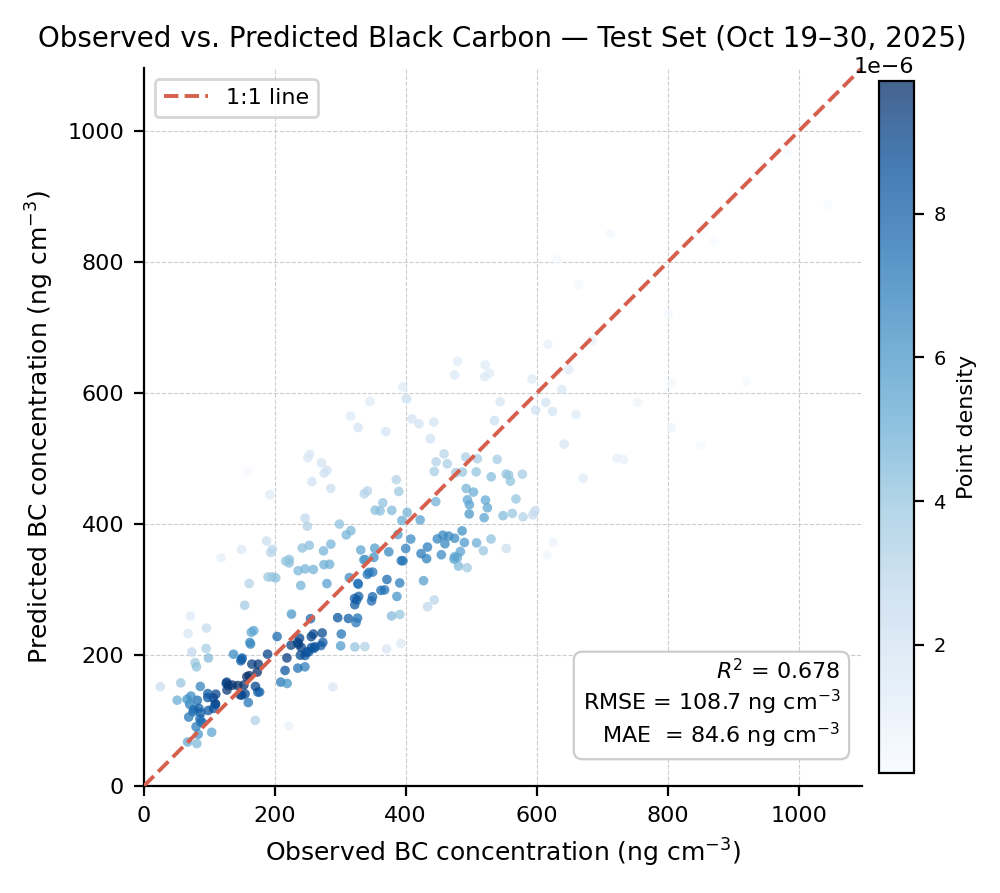
\includegraphics[width=\textwidth]{fig1_scatter.png}
    \captionof{figure}{Observed vs. predicted BC for the test set. Density-coloured scatter; dashed orange line is the 1:1 reference. Systematic underprediction above ${\sim}400$~ng~cm$^{-3}$ reflects the RF ceiling effect (leaf means cannot exceed the training-set maximum).}
    \label{fig:scatter}
\end{minipage}
\hfill
\begin{minipage}[t]{0.53\textwidth}
    \centering
    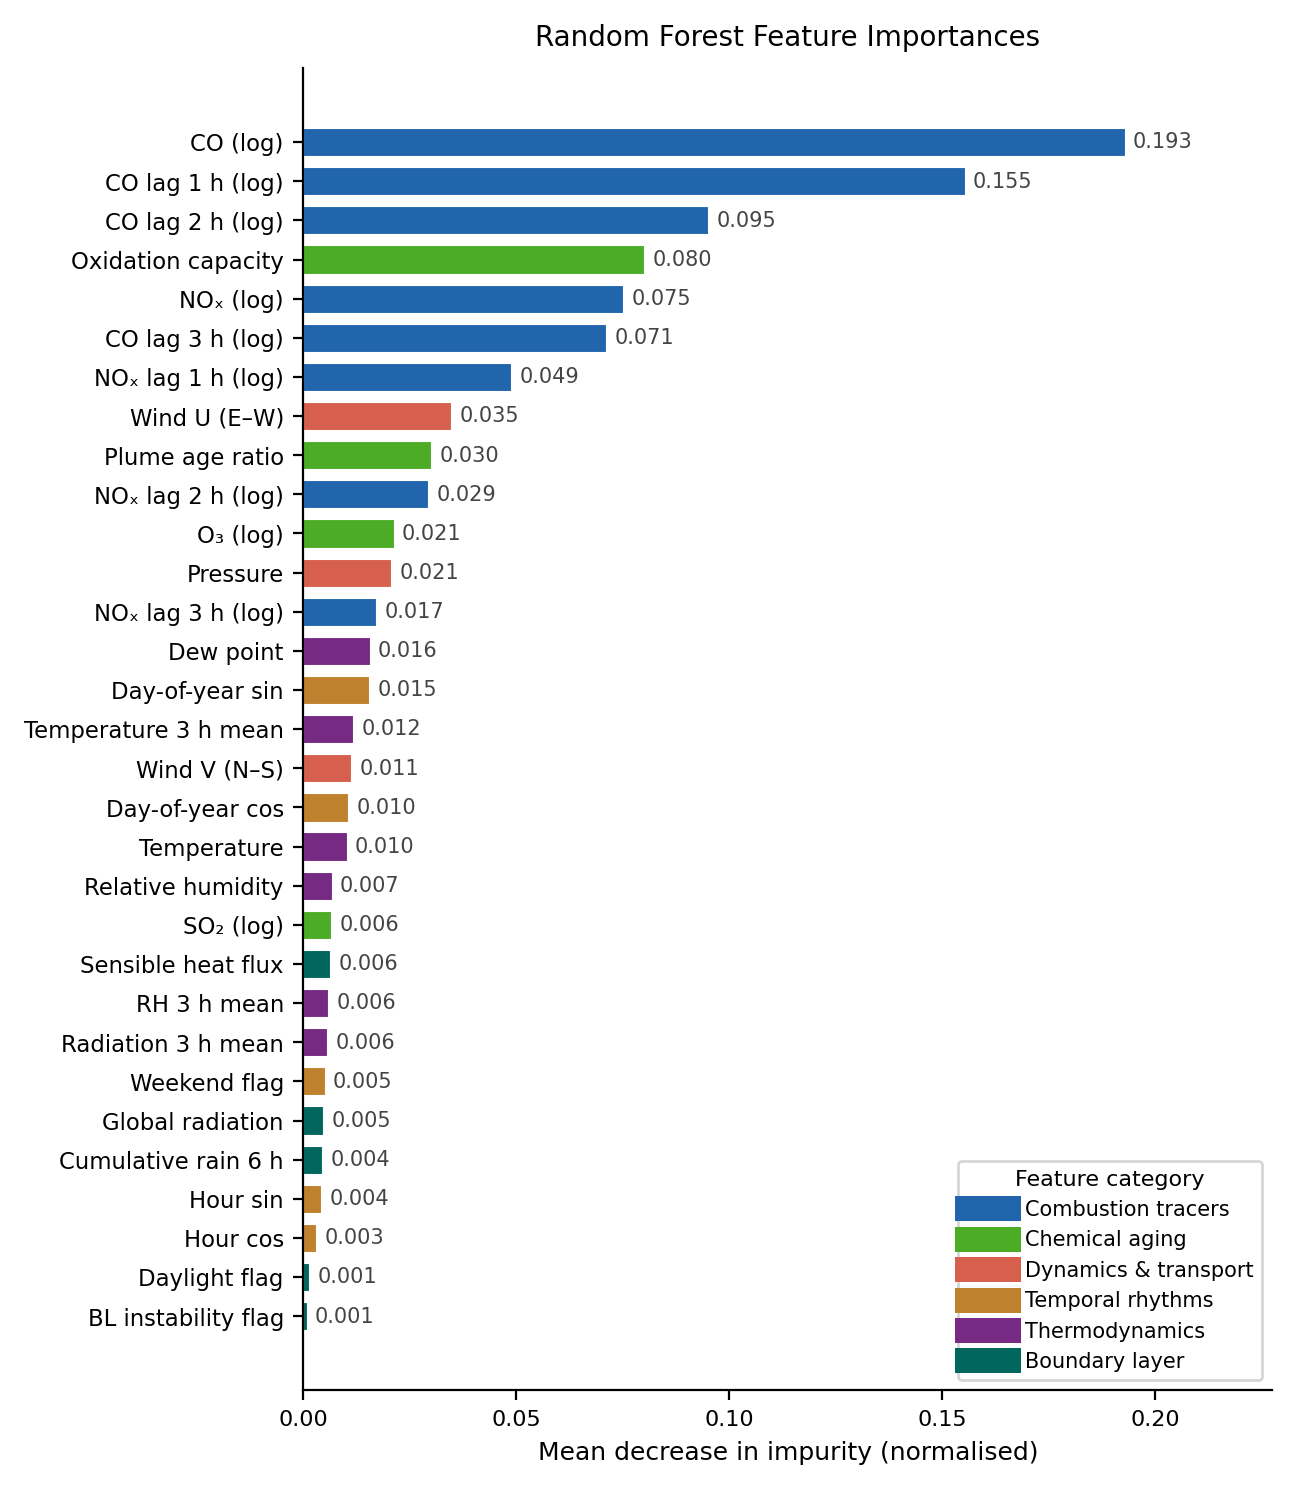
\includegraphics[width=\textwidth, height=7.0cm, keepaspectratio]{fig3_importance.png}
    \captionof{figure}{Feature importances (MDI, normalised), colour-coded by physical category. Combustion tracers (${\approx}51\%$) dominate because CO is co-emitted with BC from every combustion source. Binary BL flags rank low due to MDI bias toward high-cardinality variables \cite{james2023}.}
    \label{fig:imp}
\end{minipage}

\vspace{6pt}

\begin{figure}[H]
    \centering
    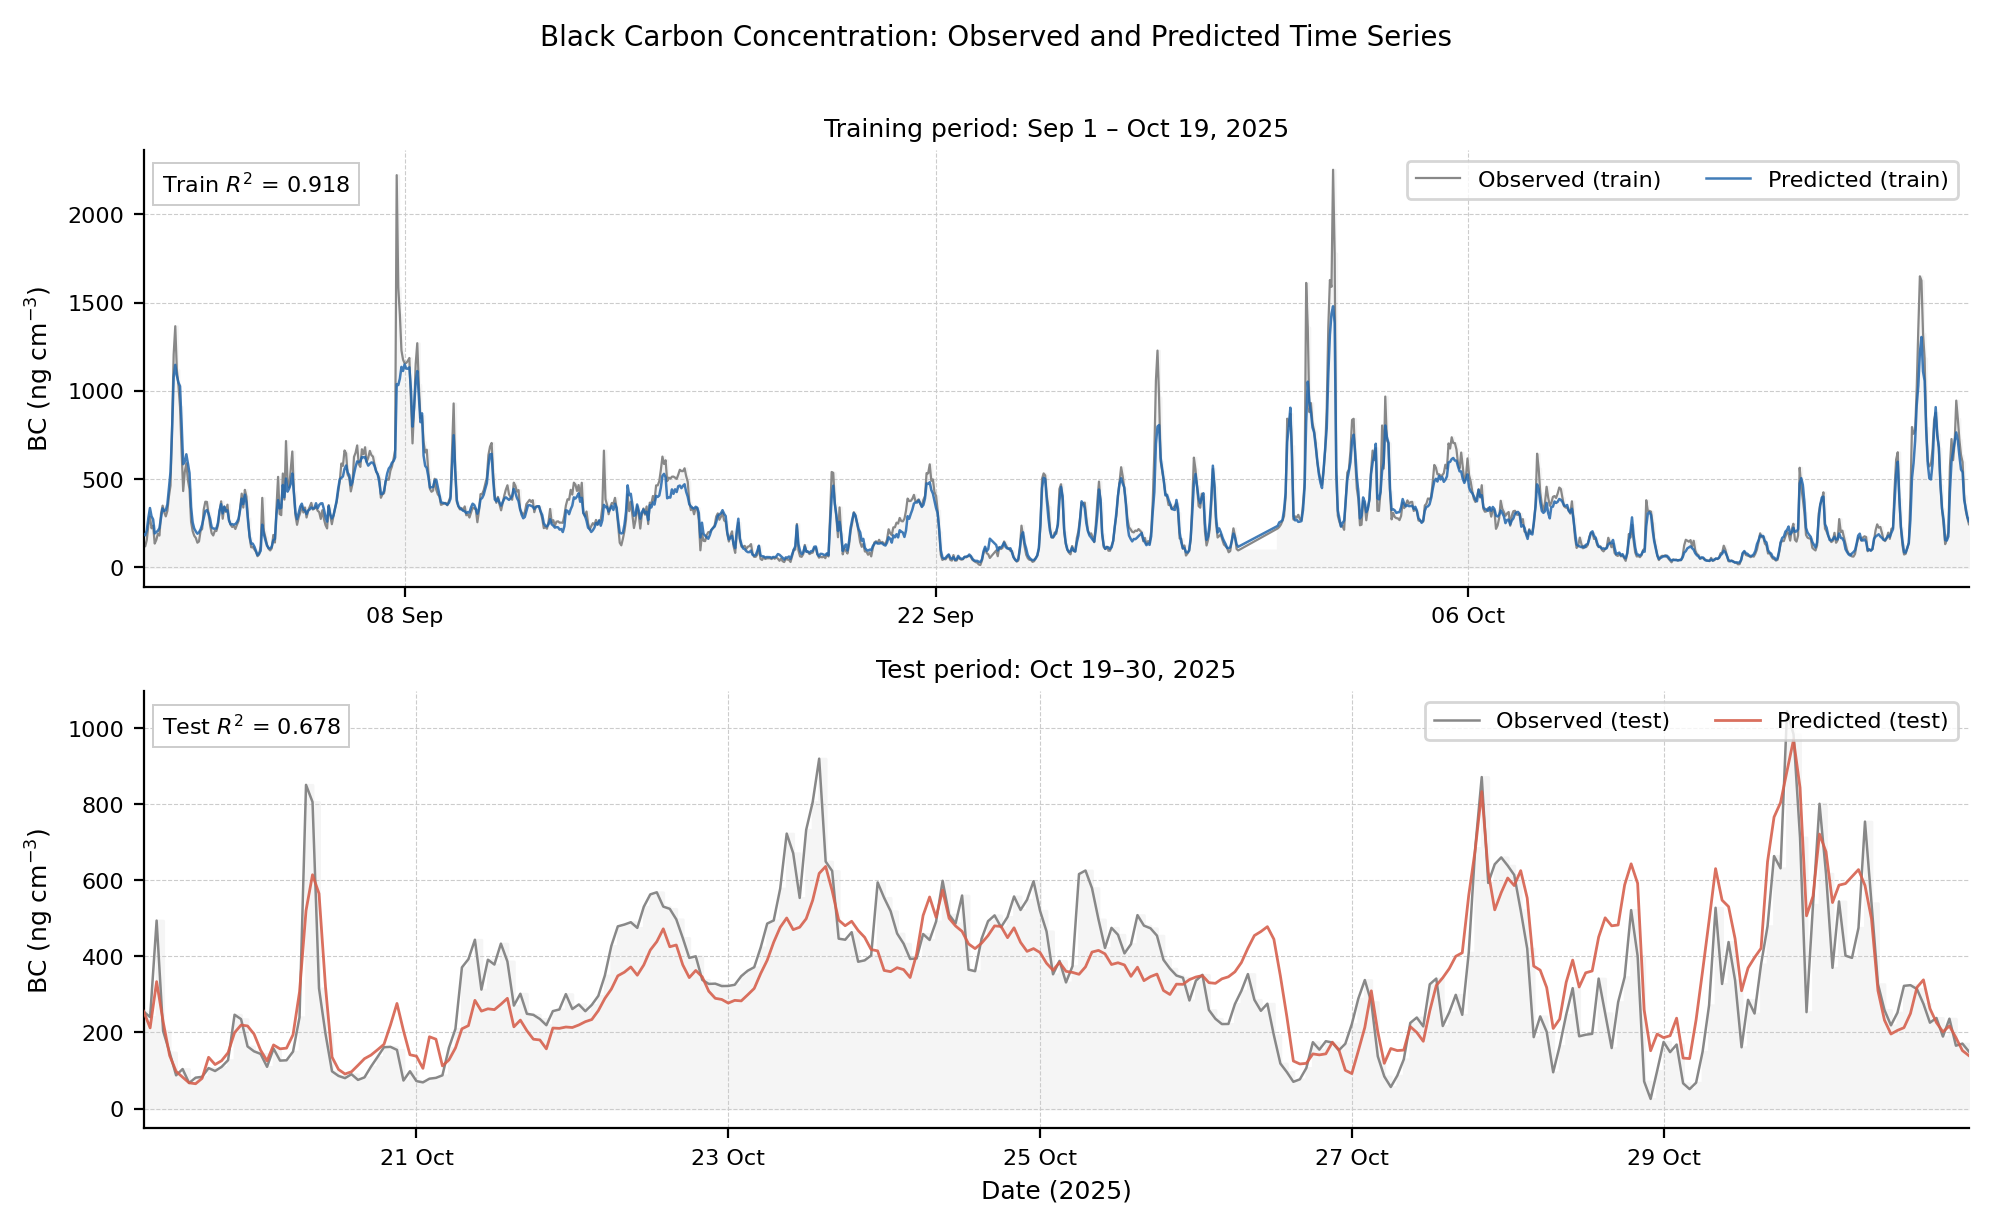
\includegraphics[width=\textwidth, height=7.0cm, keepaspectratio]{fig2_timeseries.png}
    \caption{Hourly BC concentration time series. \textbf{Upper:} training period (Sep 1 – Oct 19). \textbf{Lower:} test period (Oct 19–30). Grey shading: observed envelope; coloured lines: predictions (blue: train, orange: test). The model captures the diurnal cycle but underestimates sharp \textbf{formation events} (e.g., 22–23 Oct, 27 Oct) driven by rapid nocturnal boundary-layer collapse not resolved by 1-h predictors.}
    \label{fig:ts}
\end{figure}

Figure~\ref{fig:scatter} shows good calibration across mid-range concentrations
($50$–$300$ ng cm$^{-3}$) and consistent underprediction at the highest events
($>\!400$ ng cm$^{-3}$). Figure~\ref{fig:ts} confirms the model tracks background
variability and weekday/weekend cycles but misses rapid overnight accumulation events.

\subsection{Feature Importances}

Figure~\ref{fig:imp} shows that $\log(\mathrm{CO})$ and its three hourly lags collectively
account for ${\approx}51\%$ of total importance, followed by chemical aging proxies
(${\approx}19\%$) and dynamical features (${\approx}7\%$). The remaining categories each
contribute $<5\%$.

\section{Discussion}

\subsection{Feature Rankings and Collinearity}

The dominance of CO and its lags reflects direct co-emission of BC and CO from incomplete
combustion: CO is a near-linear proxy for fresh emission flux. Chemical aging proxies
(O$_3$/NO$_x$, CO/NO$_x$) rank next, encoding how much the plume has diluted and oxidised
since emission — older plumes have lower BC relative to CO. Wind components ($u$, $v$)
capture fetch effects: southwesterly maritime flows bring cleaner air; northeasterly
urban-sector flows carry elevated BC. Boundary-layer flags rank low in MDI, but this
reflects a known \textbf{bias of impurity-based importance toward high-cardinality continuous
features} \cite{james2023} — a binary variable that perfectly separates all samples would still
receive lower MDI than a noisy continuous one.

Several features are collinear: CO and NO$_x$ are co-emitted; temperature and dew point
share thermodynamic dependence; lag features are serially correlated by construction.
\textbf{Collinearity does not affect prediction accuracy} in a RF, because splits are
threshold-based and require no coefficient estimation. However, it distorts importance
attribution: the ${\approx}51\%$ collective share of CO and its lags overstates any single
feature's unique contribution, as importance is split unpredictably among correlated variables.

\subsection{The Covariate Shift Ceiling}
\label{sec:shift}

A two-sample Kolmogorov–Smirnov test confirms that $100\%$ of meteorological features
exhibit significant distribution shift ($p < 0.05$) between training and test sets. As shown
in Figure~\ref{fig:shift}, temperature shifts by ${\sim}8$~°C and global radiation collapses
toward zero as Helsinki approaches polar night. RF predictions are bounded by the feature
ranges seen in training \cite{james2023}: late-October atmospheric states outside the September
envelope cause decision trees to default to their nearest-seen regime, introducing systematic
extrapolation bias. This structural constraint explains why the honest $R^2$ ceiling is ${\approx}0.61$
regardless of further feature engineering; the residual ${\sim}39\%$ unexplained variance
is \textbf{physical}, not algorithmic.

\begin{figure}[H]
    \centering
    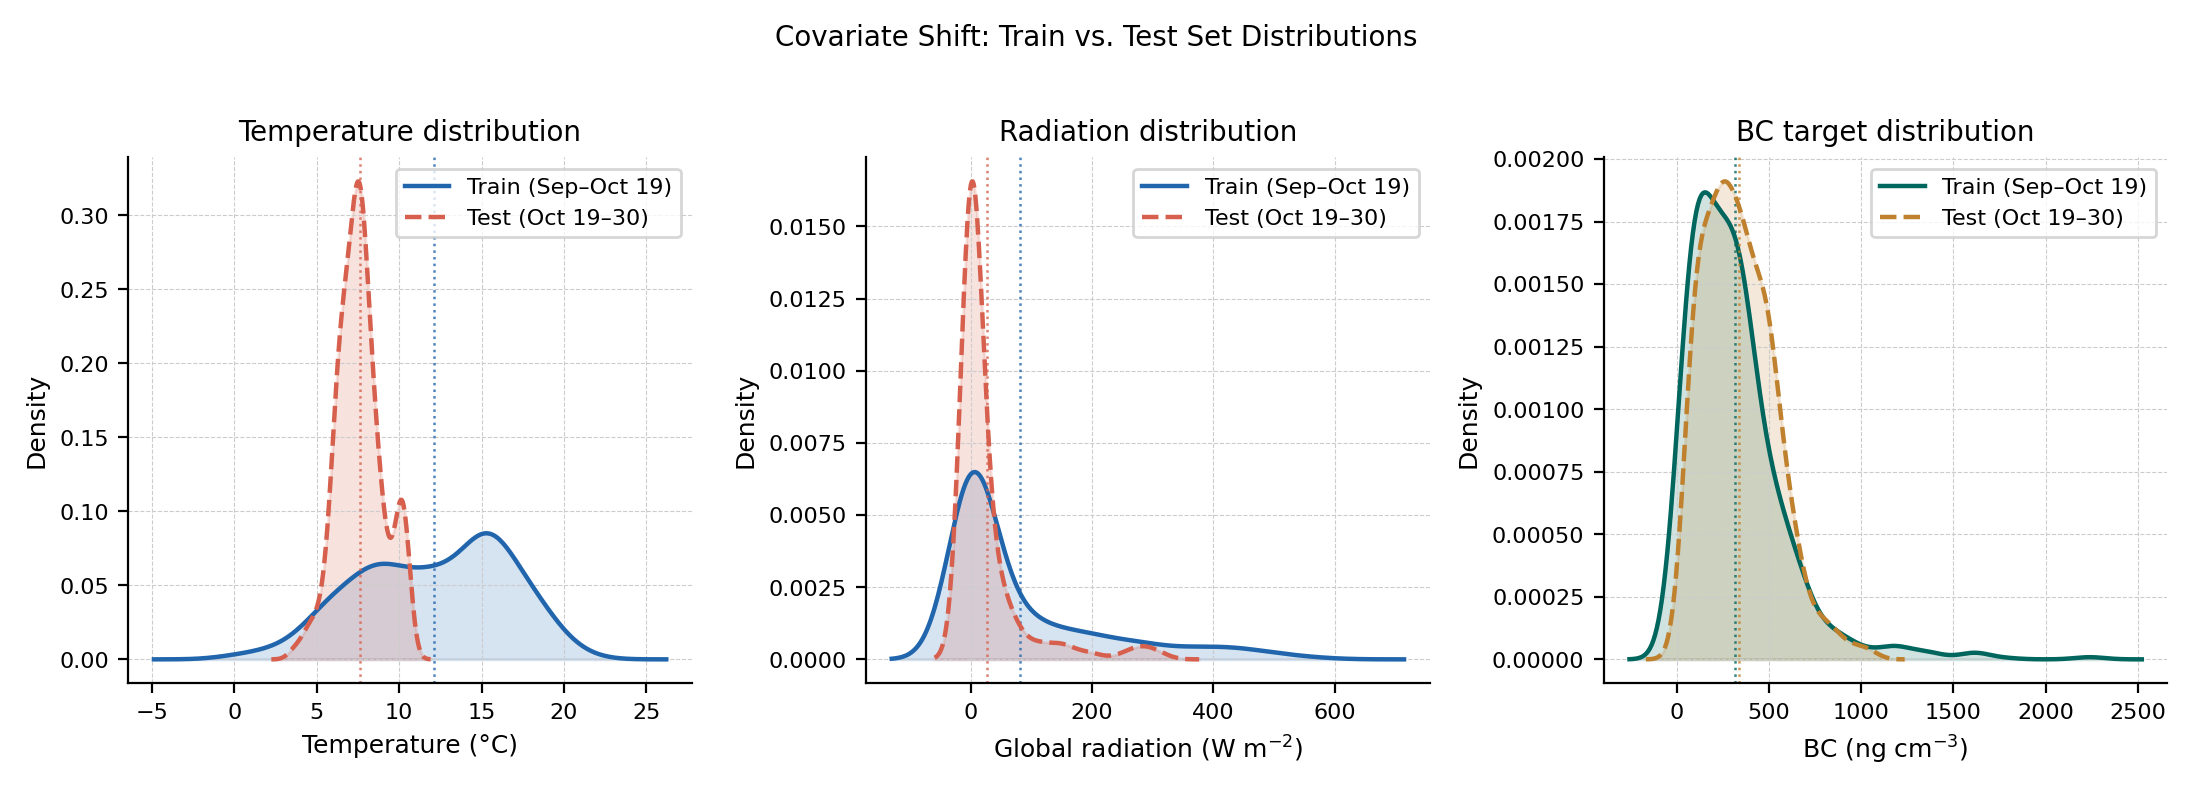
\includegraphics[width=\textwidth, height=7.0cm, keepaspectratio]{fig4_covariate_shift.png}
    \caption{KDE distributions of temperature (left), global radiation (centre), and BC (right) for training
    (blue solid) and test (orange dashed) sets. Dotted verticals are distribution means. The ${\sim}8$~°C temperature shift and near-collapse of radiation toward zero confirm a severe regime change between training and test that sets a fundamental ceiling on RF prediction skill.}
    \label{fig:shift}
\end{figure}

\section{Conclusion}


Starting from a baseline $R^2 = 0.34$, a sequence of physics-informed decisions — BC/CO
ratio target, log-transformed concentrations, temporal features, bonus boundary-layer data,
and exogenous CO/NO$_x$ lags — improved honest test performance to $R^2 = 0.61$.
The most instructive finding was that true BC autoregressive lags inflate $R^2$ by $+0.23$
through autocorrelation leakage, without any genuine predictive skill. The remaining
unexplained variance reflects a covariate shift between Helsinki's September training
and late-October polar-night test regimes — a structural limitation of partition-based
learning that transfer learning or domain adaptation would be required to overcome.

\begin{thebibliography}{9}

\bibitem{james2023}
James, G., Witten, D., Hastie, T., \& Tibshirani, R. (2023).
\textit{An Introduction to Statistical Learning with Applications in Python} (2nd ed.).
Springer. \url{https://www.statlearning.com}

\bibitem{junninen2009}
Junninen, H., Lauri, A., Keronen, P., Aalto, P., Hiltunen, V., Hari, P., \& Kulmala, M. (2009).
Smart-SMEAR: online data exploration and visualization tool for SMEAR stations.
\textit{Boreal Environment Research}, 14(4), 447--457.

\end{thebibliography}

\end{document}